\section{Тестирование программного средства}
\label{sec:principal}

При разработке программного средства на этапе перехода к использованию API Gateway возникла проблема с проксированием запросов
к API. По изначально неизвестной причине клиент возвращал ошибку CORS Policy, которую можно увидеть на рисунке \ref{fig:err}.

\begin{figure}[ht]
    \centering
    \fbox{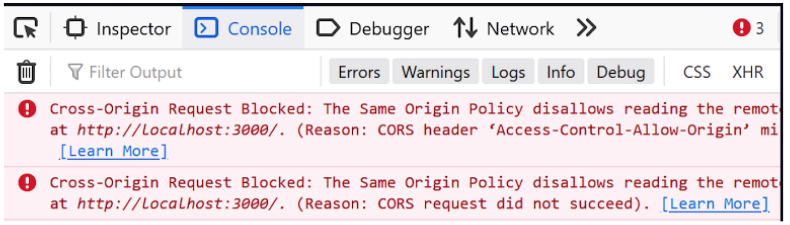
\includegraphics[width=0.75\linewidth]{\commonSecPathPrefix/sec_4/content/error.png}}
    \caption{Ошибка CORS Policy}
    \label{fig:err}
\end{figure}

После изучения проблемы и поиска её решения было выяснено, что проблема могла быть вызвана неправильной настройкой CORS в конкретном
микросервисе к которому идёт запрос. Специально для этого была написана новая конфигурация CORS, которая была добавлена в проект.
Код конфигурации можно увидеть ниже.

\begin{lstlisting}[style=CodeListing]
app.use(cors({
  origin: function(origin, callback) {
    // Разрешаем доступ для localhost и IP-адресов в диапазоне 192.168.*
    if (!origin || 
        /^http:\/\/localhost(:\d+)?$/.test(origin) || 
        /^http:\/\/192\.168\.\d+\.\d+(:\d+)?$/.test(origin)) {
      callback(null, true);  // Разрешаем запросы
    } else {
      callback(new Error('Not allowed by CORS'));  // Отказываем всем остальным
    }
  },
  methods: ['GET', 'POST', 'PUT', 'DELETE', 'OPTIONS'],
  credentials: true
}));
\end{lstlisting}

Данная конфигурация позволяет запросы только с localhost и IP-адресов в диапазоне 192.168.*. Это сделано для того, чтобы
ограничить доступ к API только для локальной сети и localhost. В дальнейшем, при необходимости, можно будет добавить другие IP-адреса.

После внесения изменений в конфигурацию CORS проблема всё ещё не была решена. Тогда было принято решение изучить журнал сообщений 
API Gateway и микросервиса, к которому идёт запрос. В журнале API Gateway не было никакой записи о запросе, что указывало на то, что
запрос не доходит до API Gateway и не обрабатывается микросервисом вовсе. Это может быть вызвано тем, что другое программное средство
перекрывает запросы.

После изучения устройства было выяснено, что в системе установлена программа WSL \cite{wslDocs} (Windows Subsystem for Linux), которая эмулирует
Linux-систему на Windows. При этом, в этой виртуальной системе был установлен сервер Apache2, который по умолчанию запускался
вместе с запуском системы. Проверить это удалось с помощью команды \texttt{sudo service apache2 status}, которая показала, что сервер
Apache2 запущен и работает. Увидеть результат команды можно ниже.

\begin{lstlisting}[style=CodeListing]
kostya@WIN-A85PV5KAN9I:/mnt/c/Users/kostyabet$ sudo service apache2 status
● apache2.service - The Apache HTTP Server
     Loaded: loaded (/usr/lib/systemd/system/apache2.service; enabled; preset: enabled)
     Active: active (running) since Sat 2025-05-17 16:10:53 +03; 4s ago
       Docs: https://httpd.apache.org/docs/2.4/
    Process: 2204 ExecStart=/usr/sbin/apachectl start (code=exited, status=0/SUCCESS)
   Main PID: 2207 (apache2)
      Tasks: 9 (limit: 14999)
     Memory: 19.3M ()
     CGroup: /system.slice/apache2.service
             2207 /usr/sbin/apache2 -k start
             2209 /usr/sbin/apache2 -k start
             2210 /usr/sbin/apache2 -k start
             2211 /usr/sbin/apache2 -k start
             2212 /usr/sbin/apache2 -k start
             2213 /usr/sbin/apache2 -k start
             2216 /usr/sbin/apache2 -k start
             2217 /usr/sbin/apache2 -k start
             2218 /usr/sbin/apache2 -k start

May 17 16:10:53 WIN-A85PV5KAN9I systemd[1]: Starting apache2.service - The Apache HTTP Server...
May 17 16:10:53 WIN-A85PV5KAN9I systemd[1]: Started apache2.service - The Apache HTTP Server.
\end{lstlisting}

При этом, Apache2 использует 80 порт, который также используется API Gateway. Это и стало причиной возникновения проблемы, а так как
Apache запускался автоматически, то он занимал порт 80 и не давал API Gateway его испрользовать. Таким образом, при попытке отправить запрос
к API Gateway, запрос перенаправлялся на Apache2, который не знал, что с ним делать и возвращал ошибку CORS Policy.
После остановки Apache2 проблема была решена и запросы начали обрабатываться API Gateway.

Для того чтобы в дальнейшем не возникало подобных проблем, было принято решение отключить автоматический запуск Apache2 при загрузке
системы. Для этого была выполнена команда \texttt{sudo systemctl disable apache2}, которая отключает автоматический запуск Apache2.
После этого, при перезагрузке системы, Apache2 не будет запускаться и 80 порт будет свободен.